\documentclass[10pt,a4paper,fleqn]{article}
\usepackage[utf8]{inputenc}
\usepackage{amsmath}
\usepackage{amsfonts}
\usepackage{amssymb}
\usepackage{graphicx}
\graphicspath{{pics/}}
\usepackage[left=2cm,right=2cm,top=2cm,bottom=2cm]{geometry}
\usepackage[hidelinks]{hyperref}
\usepackage[naustrian]{babel}
\usepackage{csquotes}
\usepackage{pbox}
\MakeOuterQuote{"}
\usepackage{array}
\renewcommand{\arraystretch}{1.8}
\begin{document}
%\setlength{\mathindent{2cm}}% you can set it back to 0cm (the default).
\begin{enumerate}
\section{Virtuelle Produktentwicklung}
\subsection{CAx - Methoden}
	\item Semi empirisch-/physikalische Modelle/Simulation\\
		P.1 F.69
		\begin{itemize}
			\item empirisch: keine mathematische Beschreibung, Annäherungen durch Messung
			\item physikalisch: physikalische Regeln und Axiome, mathematische Beschreibung eines Prozesses, numerische Lösung, Vorteil: physikalische Bedeutung
			\item semi-empritisch: empirisch+physikalisches Modell zusammen
		\end{itemize}
	\item Kirchhoff'sche Einteilung der Modellierung\\
		P.1 F.71
		\begin{center}
			\begin{tabular}{|c|c|c|}
			\hline 
			System & vernachlässigte Kräfte & angewandte Kräfte \\ 
			\hline 
			unbewegt & \pbox{20cm}{Geometrie\\ CAD} & \pbox{20cm}{(Elasto-)Statik \\ FEM, BEM} \\ 
			\hline
			bewegt & \pbox{20cm}{Kinematik \\ CAD, MBS} & \pbox{20cm}{Dynamik \\  MBS, FEM} \\ 
			\hline 
			\end{tabular} 
		\end{center}
	\item Welche Arten von Diskretisierung?\\
		P.1 F.72
			\begin{itemize}
				\item Diskretisierung von Dichte, Steifheit, Viskosität
				\item Dimensionen: unendlich $\rightarrow$ endlich
			\end{itemize}
	\item Welche Unterschiede zwischen den Typen
	
\subsection{Cax - Workflows}
	\item Workflows beschreiben, Wie/Was läuft ab.
		P.1 F.88
			\begin{itemize}
				\item DMU (Digital Mock Up)
					\begin{itemize}
						\item ditigale Dummies die eine vereinfachte Darstellung des Produktes beinhalten
						\item inkludierte Information
							\begin{itemize}
								\item Produkt Geometrie (Volumen und/oder Oberflächen)
								\item Produktstruktur
							\end{itemize}
						\item dienen Kollisionsüberprüfung, Simulation von Zusammenbau und Montage, $\dots$
						\item Als Grundlage für DMUs dienen vereinfachte 3D-CAD Daten des virtuellen Produkt Modells.
						\item Durch die Vereinfachung ist die Genauigkeit des Modells reduziert.
						\item Im DMU Prozess ist eine direkte Änderung der Geometrie nicht möglich.
						
					\end{itemize}
				\item FEM (Finite Elemente Methode)
					\begin{itemize}
						\item Genutzt für Belastungs-/, Deformations-/, Schwiungs-/, Themodynamikberechnungen
						\item FEM Berechnungen basieren auf einer angenäherten Geometrie, abgeleited von einem 3D-CAD Modell. Abhängig vom Ziel der Simulation werden verschiedene Annäherungen vorgenommen.
						\item Der Datentransfer vom 3D-CAD Modell uns FE-Programm erfolgt mit einem Diskretisierungsprozess
						\item Randbedigungen der Lasten (Kräfte, Momente, $\dots$), Einschränkungen (fixe Komponenten, Lager, $\dots$), Materialeigenschaften, Temperatur, etc. werden im FEM-Programm definiert.
						\item Nach der Simulation wird das Resultat ausgewertet. Änderungen werden an der master-Geometrie im 3D-CAD Programm und nicht in der FEM-Software vorgenommen.
					\end{itemize}
\pagebreak
				\item CFD (Computational Fluid Dynamics)
					\begin{itemize}
						\item CFD-Simulationen ermöglichen die Berechnung und Optimierung von Gas- und Flüssigkeitsströmungen.
						\item Ähnlichen den FEM-Berechnungen wird die Geometrie mit einem mesh angenähert.
						\item Datentransfer von 3D-CAD Modell zu CFD-Programm wird mit neutralen, standardisierten Datenformaten (STEP, IGES, $\dots$) vorgenommen
						\item Randbedingungen werden direkt im CFD-Programm festgelegt.
						\item Nach der Simulation wird das Resultat ausgewertet. Änderungen werden an der "Master-" Geometrie im 3D-CAD Programm und nicht in der CFD-Software vorgenommen.
					\end{itemize}
				\item MBS (Mehrkörpersimulation)
					\begin{itemize}
						\item Genutzt für kinematische Berechnungen und Optimierung des zusammengebauten und beweglichen Produkts.
						\item Das MBS-Modell basiert auf der CAD-Produkt-Struktur, wobei Körper, Verbindungen und Gelenke als Starrkörper angesehen werden. 
						\item Randbedingungen (Kräfte, Momente, Massen, Freiheitsgrade der Bewegung) werden im MBS-Programm definiert.
						\item MBS Modelle setzen sich aus vereinfachten geometrischen Elementen zusammen welche die relevanten Daten für die kinematische Berechnung beinhalten.
						\item Nach der Simulation wird das Resultat ausgewertet. Änderungen werden an der "Master-" Geometrie im 3D-CAD Programm und nicht in der MBS-Software vorgenommen.
					\end{itemize}
			\end{itemize}
	\item Prozessworkflow CAD-VR
		P.1 F.101
		\begin{itemize}
			\item Virtual Reality beschreibt eine computergenerierte Umgebung welche als Benutzerinterface fungiert.
			\item VR basierte Studien inkludieren den Nutzer in die virtuelle Umgebung
			\item Echtzeit Interaktionen der Geometrie / Funktionalität unterstützen eine Beurteilung des Modells
			\item Die Vorstellung des der Manipulierbarkeit ermöglicht eine lebensnahe Erfahrung des virtuellen Produkts.
			\item Das VRML-Datenformat (Virtual REality Modeling Language, 1994) wurde entwickelt um 3D-Modelle darzustellen und Nutzerbasierte Interaktionen zu integrieren.
			\item VRML-Daten, welche vom 3D-CAD master-Modell abgeleitet werden inkludieren vereinfachte Geometrien ausschließlich in aktueller Ausführung, ohne Verlaufsdaten.
		\end{itemize}
\subsection{Product Data Management}
	\item Was ist PDM?\\
		P.1 F.112
		PDM (Product Data Management) beinhaltet alle Aufgaben einer Organisationseinheit für die Identifizierung, Bereitstellung, Archivierung von produktrelevanten Daten während der Produktentwicklung.
	\item Warum PDM?\\
		P.1 F.113-115
		\begin{itemize}
			\item Hilft Organisationen den Daten- und Informationsfluss während des Entwicklungsprozesses zu organisieren.
			\item Die Verwaltung des Daten-, Prozess-, und Dokumentenstroms über den gesamten Lebenszyklus bilden die Grundlage für die virtuelle Produktentwicklung.
			\item Komplexe Produktstrukturen oder Variationen erzeugen zahlreiche Parameter und Informationen. Ein leistungsstarkes PDM System unterstützt den Datenaustausch zwischen den verschiedenen Phasen der Entwicklung.
		\end{itemize}
	\item Concepts of the virtual product development\\
		P.1 F.116
\pagebreak
	\item Nennen Sie Daten die in einem PDM System verwaltet werden können
		\begin{itemize}
			\item Geometriedaten
			\item 2D-Zeichnungen
			\item Produktstruktur
			\item Ergebnisse von Analysen
			\item Dokumente
		\end{itemize}
	\item Hauptfunktionen PDM\\
		P.1 F.119
		\begin{itemize}
			\item Produktstruktur-management
			\item Workflow-management
			\item Projekt-management
			\item Dokument-management
			\item Klassifikation / Varianten
			\item Beziehungen untereinander: Personen $\Leftrightarrow$ Prozesse $\Leftrightarrow$ Teile $\Leftrightarrow$ Dokumente $\Leftrightarrow$ Daten
		\end{itemize}
\newpage
\section{Computer-Aided Design (CAD)}
\subsection{Geometrical representation models in CAD}
	\item Element Typen\\
		P.2 F.13-29
	 	\begin{itemize}
	 		\item Drahtgitter: Punkte und Kurven definieren 2D- und 3D-Objekte
	 		\item Flächen: Ebene und gewölbte Flächen im $\mathbb{R}^3$
	 		\item Solid: Ermöglicht komplette geometrische Darstellung von realen Produkten in virtueller Umgebung
	 			\begin{itemize}
	 				\item Schalengeometrie: geschlossene Schalten $\rightarrow$ Solid
	 				\item Unterscheidung zwischen Innen und Außerhalb des Solids
	 				\item Definition Materialeigenschaften (für Simulationen)	 			
	 			\end{itemize}
	 		\item Hybride Modelle
	 	\end{itemize}
	 \item Was ist ein Skelettmodell\\
	 	P.2 F.14
	 	s.o.
	 \item Wie wird es angewandt?
	 \item Anwendung von Bool'schen Operationen bezogen auf Produktion\\
	 	P.2 F.25,27
	 	\begin{itemize}
	 		\item Vereinigungs Operator (A$\cup$B)
	 		\item Subtraktions Operator (A$ - $B)
	 		\item Schnittmenten Operator (A$\cap$B)
	 	\end{itemize}
	 	Anstatt nach und nach das gewünschte Objekt zu erstellen wird das Negativ konstruiert und von einer Grundform abgezogen. Zur Zeit übliche Vorgangsweise.
	
\subsection{Parametric-associative design}
	 \item Was ist parametrische Konstruktion\\
	 	P.2 F.31
	 	\begin{itemize}
	 		\item parametrische Konstruktion verbindet geometrische Objekte mit geometrischen Beschränkungen und Maßangaben
	 		\item Veränderungen der Geometrie durch Änderung der Eingabewerte der dazugehörigen Beschränkungen
	 		\item Assoziative Konstruktionsoperationen schließen Beziehungen und Abhängigkeiten zwischen geometrischen Objekten direkt ein. Diese geometrischen Verbindungen sind als Teil des Kontruktionsprozesses definiert und erstellen Eltern-Kind Beziehungen oder Verhältnisse mehrerer Geometrien zum selben Parameter, zu den selben Parametern.
	 		\item Moderne CAD Systeme bieten Mehr-Modell-Verknüpfungen, welche die Definition assoziativer Funktionalität zwischen (vormals unabhängigen) Teilen in Baugruppen anbietet.
	 	\end{itemize}
\pagebreak
	 \item Parametrische Beschreibung\\
	 	P.2 F.32
	 	\begin{itemize}
	 		\item Virtuelle Produkt
	 			\begin{itemize}
	 				\item Parameter
	 					\begin{itemize}
	 						\item geometische Parameter (Koordinaten, Dimensionen, $\dots$)
	 						\item Material Parameter (Dichte, Festigkeit, Rauheit, $\dots$)
	 						\item Technologische Parameter (Vorschub, Schnittgeschwindigkeit, $\dots$)
	 					\end{itemize}
	 				\item Beschränkungen
	 					\begin{itemize}
	 						\item geometische Beschränkungen (absolute und relative Positionen, Orientierungen, $\dots$)
	 						\item Ingenieurliche(?) Beschränkungen (funktional / logisch)
	 					\end{itemize}
	 				\item strukturelle Parameter
	 					\begin{itemize}
	 						\item Struktur der Montagegruppen
	 						\item Struktur der Teile
	 					\end{itemize}
	 			\end{itemize}
	 	\end{itemize}
	 \item Herausforderungen bei parametrischer Konstruktion\\
	 	P.2 F.43
	 	\begin{itemize}
	 		\item Ingenieure tendieren zu unterschiedlicher Implementation von Methoden
	 		\item parametrische Modelle werden komplexe, intrasparente Strukturen
	 		\item Mehr-Modell-Verknüpfungen (Assoziationen zwischen Modellen) können zu Organisationsproblemen führen
	 		\item erhöhtes Datenvolumen, vor allem bei unterschiedlichem Datenstand
	 		\item komplexe Verknüpfungen führen zu umfangreicher Datenverarbeitung
	 		\item komplexe Verknüpfungen führen zu "Referenzierung im Kreis" $\rightarrow$ logische Probleme
	 		\item parametrische Modelle enthalten Expertenwissen $\rightarrow$ Problem des Wissenstransfer
	 	\end{itemize}
\subsection{Knowledge based design}
	\item Was sind Wissensträger?\\
		P.2 F.46
		\begin{itemize}
			\item Skizzen
			\item Parameter, Beziehungen, Regeln, Schemen
			\item Benutzer-features
			\item Modell Verlauf
			\item Vorlagen Modelle
			\item Startup models
			\item Produktstruktur
			\item Attribute und Anmerkungen
			\item DMU - Funktionalität (z. B. kinematische Simulation)
			\item $\dots$
		\end{itemize}
	\item Welche Arten von Wissensträger gibt es?\\
		P.2 F.47
		\begin{itemize}
			\item Modelle mit fixer Geometrie
			\item Modelle mit variabler Geometrie
			\item Integration von mathematischen / logischen Beziehungen
			\item automatisierte Abläufe für die geometrische Erzeugung oder berechnende Prozeduren
			\item interaktive Programme
		\end{itemize}
	\item Was ist eine Template?
%	\item Adapive Modelle z.B. 
	\item Levels of knowledge content in CAD models\\
		P.2 F.49\\
		Ansteigender Wissengehalt\\
		\begin{tabular}{l|l}
			Art des CAD Modells & Anwendungsbeispiel \\ 
			\hline 
			\pbox{20cm}{1. neutrale Datenformate \\ \mbox{}\hspace{0.4cm}(IGES, STEP, etc.)} & Virtualisierung \\ 
			\pbox{20cm}{2. reduziertes Geometriemodelle \\ \mbox{}\hspace{0.4cm}(z. B. teilweise vereinfachte Geometrie) } & DMU, Zulieferkette \\ 
			\pbox{20cm}{3. detaillierte Geometriemodelle \\ \mbox{}\hspace{0.4cm}(z. B. isolierte Geometrie)} & Zeichnungen, Simulationen \\ 
		 	4. parametrische Modelle & Entwurf, Entwicklung \\ 
			5. Nutzer features & Design-Prozess \\ 
			6. Vorlagenmodelle & Fortgeschrittenes design \\ 
			7. Skelett- und adaptive Modelle  & Design in context \\ 
		\end{tabular}
\subsection{Assembling and product structures}
	\item Welche Elemente sind in Baumstruktur (Übersicht)\\
		P.2 F.51
		\begin{itemize}
			\item Teil-Nummer / Name der Komponente
				\begin{itemize}
					\item Axen Systeme
					\item Parameter / Beziehungen
					\item Eingabedaten / externe Geometrien
						\begin{itemize}
							\item Styling Surface
							\item Adapter Geometry
							\item externe Begrenzungen, etc.
						\end{itemize}
					\item Referenzelemente
						\begin{itemize}
							\item Referenzpunkte, -linien, -flächen
							\item Referenzskizzen, -gitterelemente
						\end{itemize}
					\item Standards und Informationen
						\begin{itemize}
							\item Demold
							\item Informationen bzgl. Produktion
							\item Anmerkungen, etc.
						\end{itemize}
					\item Definition der Geometrie
						\begin{itemize}
							\item Part Geometrie
								\begin{itemize}
									\item grundlegende Geometrie
									\item Wellen/Furchen
									\item Flanschen
									\item Taschen
									\item etc.
								\end{itemize}
							\item Schnittflächen
							\item geschnittene Teilgeometrie
						\end{itemize}
					\item Veröffentlichung der finalen Oberfläche
					\item Berechnungen und Maße
						\begin{itemize}
							\item Gewicht, Fläche, etc.
						\end{itemize}
				\end{itemize}
		\end{itemize}
	\item Wozu?
\subsection{Aufbau und Produktstruktur}
	\item Was wird bei einer Baumgruppenkonstruktion gemacht?\\
		P.2 F.56\\
		Aufbaudesign beinhaltet die Organisation und Verknüpfung von zahlreichen Komponenten und Modulen von Produkten\\
		Aufbaudesign behandelt \vspace{-0.3cm}
			\begin{itemize}
				\item Positionierung von Komponenten
				\item Definition von Verhältnis und Verknüpfungen zwischen Komponenten
				\item Organisation von Mehr-Modell-Verknüpfungen
				\item Organisation von Parameterstrukturen
				\item Bereitstellung von Geometrie und Struktur für nachfolgende DMU-Prozesse
				\item Bereitstellung von Geometriedaten für Montagebasierte-Simulation (z. B. MBS)
				\item Interaktion mit PDM-Systemen
			\end{itemize}
	\item Wie werden komplexe Baugruppen organisiert? \\
		P.2 F.59\\
		Einteilung in Hierarchie-Ebenen\\
		\begin{center}
			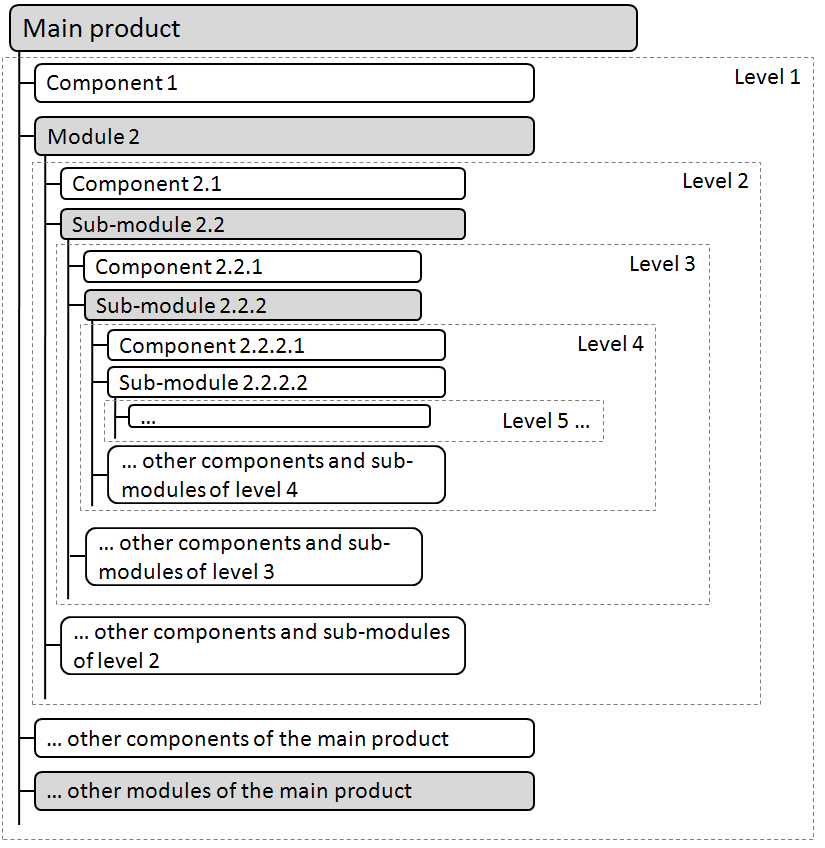
\includegraphics[scale=0.3]{hirarchie.png}
		\end{center}		
	\item Methoden der Positionierung\\
		P.2 F.61
		\begin{enumerate}
			\item Durch Beschränkungen
			\item Durch ein oder mehrerer Skelettmodelle
			\item Relativ zu einem Referenzkoordinatensystem
		\end{enumerate}
\pagebreak
\section{Virtuelle Entwicklung mechatronischer Produkte}
\subsection{Einleitung - Mechatronik}
	\item Was ist Mechatronik?\\
		P.3 F.3-4\\
		Die Mechatronik beschreibt technische Systeme, welche sich aus mechanischen, elektrischenund elektronischen Komponenten zusammensetzen.
	\item Randbedingung, was ist kritisch\\
		P.3 F.8\\
			\begin{center}
				\begin{tabular}{|l|l|}
					\hline 
					Äußere Randbedingungen & Innere Randbedingungen \\ 
					\hline 
					\pbox{20cm}{kurze Lebensdauer \\ mechatronischer Produkte/ \\ schneller Modellwechsel} & \pbox{20cm}{fehlende domäneübergreifende \\ Spezifikation der Produkte \\ (Beschreibungssprache)} \\ 
					\hline 
					\pbox{20cm}{hohe Zahl von Varianten \\ (Kundenwünsche) } & \pbox{20cm}{unterschiedliche Entwicklungsmethoden \\ und IT Werkzeuge in den Domänen  } \\ 
					\hline 
					\pbox{20cm}{Produkte müssen zuverlässiger \\ werden (Wettbewerb) } & \pbox{20cm}{ Fehlende gemeinsame Simulatino \\ der zu entwickelnden Produkte } \\ 
					\hline 
					\pbox{20cm}{ Entwicklungskosten müssen \\ gesenkt werden (Wettbewerb) } &  Hohe Produktkomplexität \\ 
					\hline 
				\end{tabular}
			\end{center}
	\item V-Modell!\\
		P.3 F.15\\
		\begin{center}
			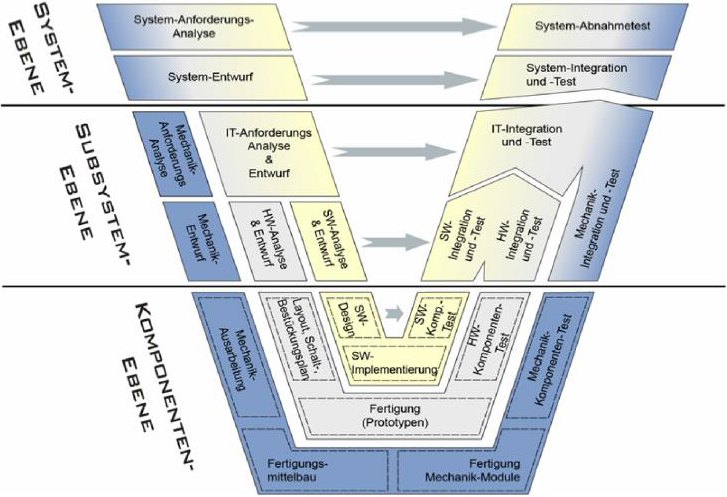
\includegraphics[scale=0.5]{v.png}
		\end{center}
\subsection{Komponenten mechatronischer Systeme}
	\item Übersicht Komponenten\\
		P.3 F.17
		\begin{center}
			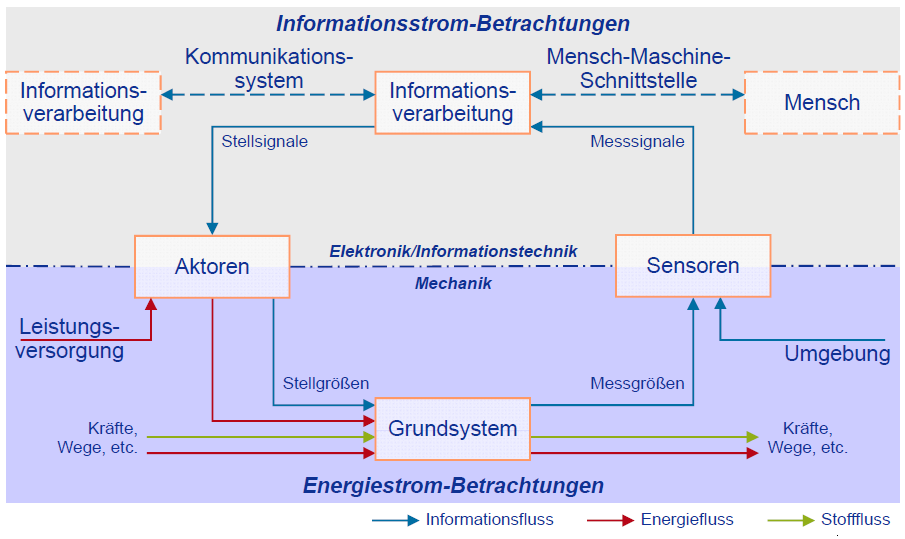
\includegraphics[scale=0.4]{komponenten.png}
		\end{center}
	\item Aufbau Regelkreis\\
		P.3 F.18\\
		\begin{center}
			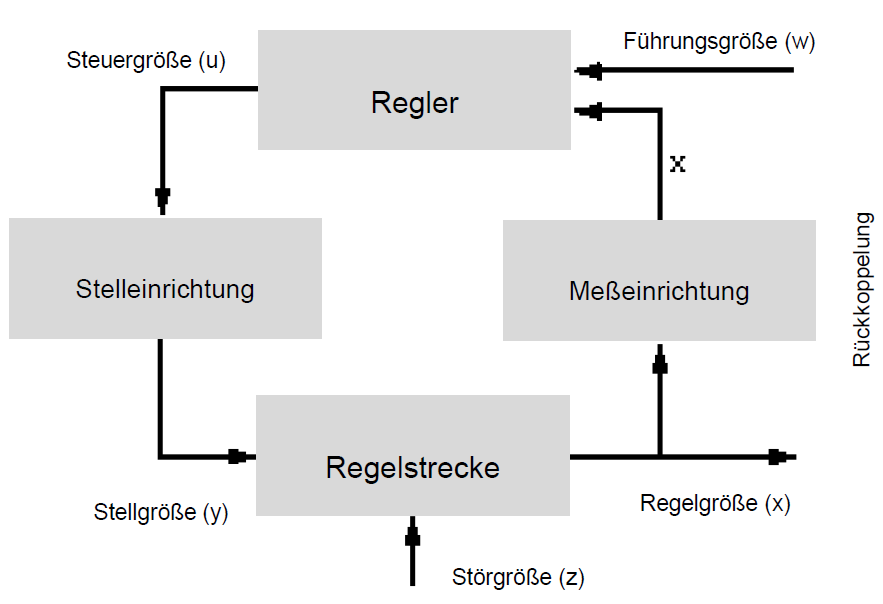
\includegraphics[scale=0.5]{regelkreis.PNG}
		\end{center}		
	\item Definition Aktor, Sensor, Prozessdatenverarbeitung
		\begin{itemize}
		 	\item Aktoren: P.3 F.19-23\\
		 		Technisch gesehen versteht man unter einem Aktor die Zusammenschaltung eines Energiewandlers mit einem Leistungsstellglied.\\
		 		Das Leistungsstellglied verbindet die eingehende Energie (in der Regel elektrische Energie) mit dem Stellsignal. Es entsteht eine modulierte Energie, die vom Wandler in die Energieart der Stellgröße (meist mechanische Energie) transformiert wird.\\
				In mechatronischen Systemen stellen Aktoren das Bindeglied zwischen der Informationsverarbeitung und dem mechanischen Grundsystem dar.
\pagebreak
		 	\item Sensoren: P.3 F.24-28\\
		 		Sensoren wandeln die zu messenden physikalischen oder chemischen Größen in elektrische Signale um.\\
				Ein Signal stellt in diesem Sinne eine zeitvariable, physikalische oder chemische Zustandsgröße (z.B. Druck, Temperatur, Kraft, usw.) als zeitliche Abfolge von Messwerten dar.\\
				Funktional besteht ein Sensor aus
					\begin{itemize}
						\item einem Sensorelement, das die Messgröße in ein elektrisches Signal umwandelt, und
						\item einer Signalverarbeitung, die ein genormtes elektrisches Ausgangssignal liefert
					\end{itemize}
				Somit sind Sensoren Komponenten, welche ein im allgemeinen nicht elektrisches Signal (Messignal) in ein elektrisches Signal umwandeln.
		 	\item Prozessdatenverarbeitung: P.3 F.30\\
				Die Verarbeitung von Prozessdaten erfolgt in den meisten Fällen in Mikroprozessoren. Hier werden in Abhängigkeit der Komplexität der mechatronischenSysteme verschiedene Anforderungen gestellt. \\
				\textbf{Echtzeitdatenverarbeitung:} Systeme sind echtzeitfähig wenn sie in der Lage sind, unabhängig von Art und Umfang des gerade bearbeiteten Problems auf ein zu beliebiger Zeit auftretendes Ereignis höherer Dringlichkeit spätestens nach Ablauf einer definierbaren maximalen Reaktionszeit $\text{t}_{\text{Rmaxin}}$ programmierbarer Weise zu reagieren. Die Reaktionszeit bezeichnet dabei die Zeit, die der Rechner benötigt bis der Task gerechnet werden kann.\\
				\textbf{Multitasking:} Dieses Verfahren ermöglichen die Berücksichtigung mehrerer Prozesse/ Threads durch den Prozessor. Die Verwaltung einer hohen Zahl von Tasks muss für die höchstpriorisierten Tasks ohne Auswirkungen bleiben. Synchronisationsmechanismen, die den Tasks erlauben, ihre Aktivitäten gegenseitig abzustimmen, müssen optimiert werden.\\
				\textbf{Multiprocessing:} Es gibt 3 Kategorien von Multiprocessing		
					\begin{itemize}
						\item Heterogene Architekturen: Die Prozessoren übernehmen verschiedenartige Aufgaben und sind oft auch nicht vom gleichen Typ.
						\item Lose gekoppelte Architekturen: Die Prozessoren besitzen eigene Speicher, sind jedoch über schnelle Datenverbindungen gekoppelt.
						\item Eng gekoppelte Architekturen: Die Prozessoren sind gleichartig und teilen sich auch den Speicherbereich.
					\end{itemize}
		 \end{itemize}
\subsection{Hardware in the Loop (HiL) / Software in the Loop (SiL)}
	\item Was ist SiL/HiL, wie wird es angewandt.\\
		P.3 F.32-37
		\begin{itemize}
			\item \textbf{Hardware in the Loop (HiL)}
				Hardware in the Loop (HIL) ist eine Methode zum Testen und Absichern von eingebetteten Systemen, zur Unterstützung während der Entwicklung sowie zur vorzeitigen Inbetriebnahme von Maschinen und Anlagen.

				Bei Hardware in the Loop (HIL) wird ein reales System (z.B. reales elektronisches Steuergerät oder reale mechatronische Komponente) über seine Ein- und Ausgänge an ein angepasstes Gegenstück (HIL-Simulator) angeschlossen. Dabei übernimmt der HIL-Simulator die Nachbildung der realen Umgebung des Systems durch virtuelle Methoden.
				
				Bei HIL für eingebettete Systeme wird das zu steuernde System (z.B. Auto) über Modelle simuliert, um die korrekte Funktion des zu entwickelnden Steuergerätes (z.B. Motorsteuergerät) zu testen. Die HIL-Simulation muss meist in Echtzeit ablaufen und wird in der Entwicklung benutzt, um Entwicklungszeiten zu verkürzen und Kosten zu sparen.
				
				Insbesondere lassen sich wiederkehrende Abläufe simulieren. Dies hat den Vorteil, dass eine neue Entwicklungsversion unter den gleichen Kriterien getestet werden kann wie die Vorgängerversion. Somit kann detailliert nachgewiesen werden, ob ein Fehler beseitigt wurde oder nicht.
				
				Der HIL-Simulator besteht also aus einem Rechner, der die Echtzeitbedingungen der jeweiligen Anwendung erfüllen kann (zunehmend auch PC-basiert), digitale und analoge Ein-und Ausgabe-Schnittstellen zum Steuergerät und Ersatzlasten, die der steuergeräteinternen Endstufendiagnose simulieren, dass alle Aktuatoren korrekt angeschlossen seien.
				
				Die Tests an realen Systemen lassen sich dadurch stark verringern und zusätzlich lassen sich Systemgrenzen ermitteln, ohne das Zielsystem (z.B. Auto und Fahrer) zu gefährden.
				
				Die HIL-Simulation ist immer nur eine Vereinfachung der Realität und kann den Test am realen System deshalb nicht ersetzen. Falls zu große Diskrepanzen zwischen der HIL- Simulation und der Realität auftreten, sind die zugrundeliegenden Modelle in der Simulation zu stark vereinfacht. Dann müssen die Simulations-Modelle weiterentwickelt werden.
				
				Die Entwicklung mittels HIL ist mittlerweile in verschiedenen Branchen der mechatronischen Produktentwicklung vertreten, z.B. in der Automobilindustrie, der Luft- und Raumfahrt, sowie im Maschinen- und Anlagenbau.
				
				Beispiel für eine angewandte HIL-Entwicklungsmethodik in der Automobilindustrie. Das HIL-System simuliert dabei die Umgebung (Fahrzeug, Reifen, Straße) des realen Steuergerätes.
			
			\item \textbf{Software in the Loop (SiL)}
				Bei der Methode Software in the Loop (SIL) wird im Gegensatz zum HIL keine besondere Hardware eingesetzt. Das erstellte Modell der Software wird lediglich in den für die Zielhardware verständlichen Code umgewandelt (beispielsweise von einem MATLAB/ Simulink-Modell). Dieser Code wird auf dem Entwicklungsrechner zusammen mit dem simulierten Modell ausgeführt, anstatt wie bei Hardware in the Loop auf der Zielhardware zu laufen. Es handelt sich dabei also um eine Methode, die vor dem HIL anzuwenden ist.
				
				Vorteile von SIL sind unter anderem, dass die Zielhardware noch nicht feststehen muss, und dass die Kosten aufgrund der fehlenden Simulationsumgebung weitaus geringer ausfallen. Das hier benutzte Modell der Strecke kann auch beim HIL weiter verwendet werden, und somit die einzelnen Testläufe miteinander verglichen werden.
				
				Nachdem sowohl der Prozess, als auch die Regelung / Steuerung in der Simulation vorliegen, sind verschiedene Testszenarien denkbar. Wird der Regelungsalgorithmus unter Verwendung einer geeigneten Codegenerierung auf eine leistungsfähige Simulations-Hardware übertragen, kann der reale Prozess mit dem Regelungsalgorithmus betrieben werden, ohne, dass bereits an dieser Stelle ein Mikrokontroller oder Ähnliches mit den einhergehenden Nachteilen (Speicherplatzbeschränkung, begrenzte Prozessorleistung) eingesetzt werden müsste $\rightarrow$ "Software in the Loop".
		\end{itemize}
\subsection{Computer aided software engineering (CASE)}
	\item Upper-/Lower CASE\\
	P.3 F.39-41
		Unter Computer-aided software engineering (CASE) versteht man den intensiven Einsatz IT-gestützter Werkzeuge für die Umsetzung einer Software-Konzeption. Ziel ist es, Software möglichst vollständig automatisiert aus fachlichen Beschreibungen (Vorgeben) zu erstellen.
		
		CASE-Tools sind Programme, die den Software-Ingenieur bei der Planung, dem Entwurf und der Dokumentation seiner Arbeitsergebnisse (Software) unterstützen. Ein wichtiger Bestandteil von CASE-Tools ist eine grafische Notationsweise, die der Visualisierung der Architektur des Software-Systems dient.

		CASE-Tools sind oft in Entwicklungsumgebungen (IDEs) integriert; manchmal sind es auch eigenständige Applikationen, deren Fokus vollständig auf CASE liegt (ohne dabei die anderen typischen Elemente einer Entwicklungsumgebung anzubieten).\\
\newpage
		\textbf{Upper-CASE}-Tools unterstützen die frühen (oberen) Phasen der IS-Entwicklung. Sie erlauben die rechnergestützte konzeptionelle Modellierung, beispielsweise mit Hilfe von Entity-Relationship-, \mbox{Funktionshierarchie-,} Datenflußdiagrammen usw.\\
		\begin{center}
			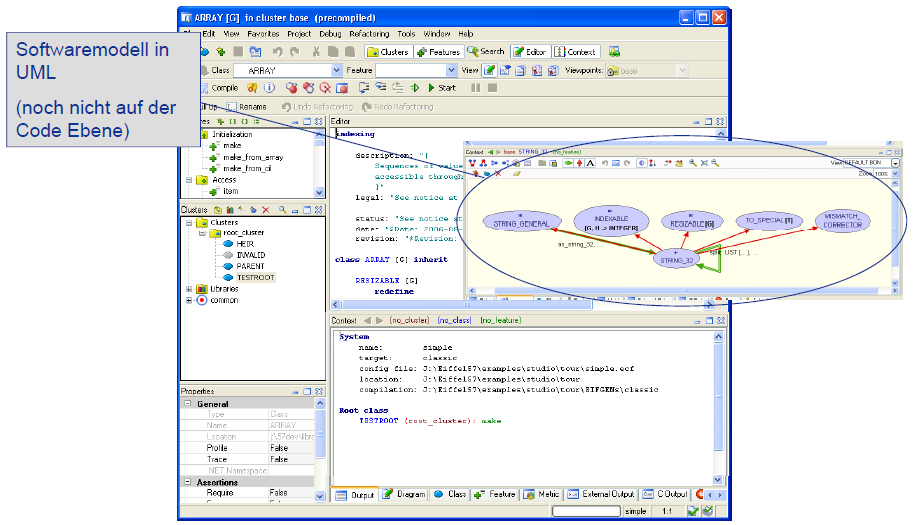
\includegraphics[scale=0.45]{UpperCASE.png}
		\end{center}				
		\textbf{Lower-CASE}-Tools bestehen aus einem Satz von Programmgeneratoren, die aufgrund der erfassten Modelldaten selbständig den benötigten Programmcode für die gewünschten Anwendungen erzeugen.\\
		\begin{center}
			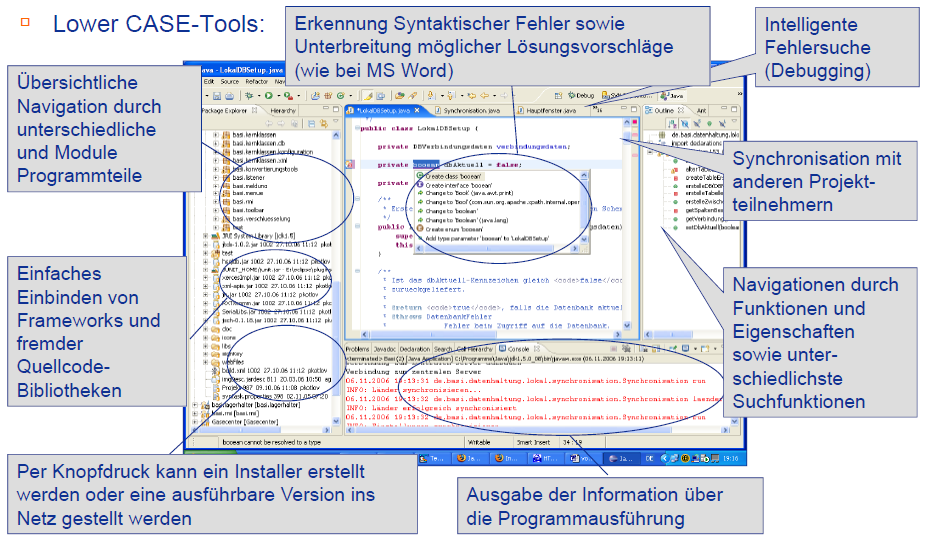
\includegraphics[scale=0.45]{LowerCASE.png}
		\end{center}		
\end{enumerate}
%
%\newpage
%
%\begin{enumerate}
%	\item Nennen Sie die Abschnitte eines typischen Produktlebenszyklus.
%	\item Welche Prozesse finden in den einzelnen Phasen eines Produktlebenszyklus statt?
%		\begin{itemize}
%			\item Anforderungen
%				\begin{itemize}
%					\item Anforderungsanalyse
%					\item Anforderungserfassung
%				\end{itemize}
%			\item Produktplanung
%				\begin{itemize}
%					\item Programm-/Portfolio-Planung
%					\item Projektplan-, Team- \& Kosten-Festlegung
%				\end{itemize}
%			\item Entwicklung
%				\begin{itemize}
%					\item Mechanische Konstruktion
%					\item Elektrokonstruktion
%					\item Softwareentwicklung
%					\item Simulation, DMU/PMU
%					\item Absicherung/Versuche
%					\item Dokumentation
%				\end{itemize}
%			\item Prozessplanung
%				\begin{itemize}
%					\item Prozessplanung
%					\item Analgenplanung
%					\item Anlagenentwicklung
%					\item Einkauf
%					\item Simulation/Versuche
%				\end{itemize}
%			\item Produktion
%				\begin{itemize}
%					\item Herstellung
%					\item Zusammenbau
%					\item Qualitätssicherung
%				\end{itemize}
%			\item Betrieb
%				\begin{itemize}
%					\item Vertrieb
%					\item Service
%					\item Wartung und Reparatur
%				\end{itemize}
%			\item Recycling
%				\begin{itemize}
%					\item Recycling
%				\end{itemize}
%		\end{itemize}
%	\item Warum sollten die Entwicklungszeiten möglichst kurz sein?
%	\item Welchen Einfluss hat die Produktkomplexität auf die Produktentwicklung?
%	\item Warum spielt die frühe Phase in der Produktentwicklung eine entscheidende Rolle?
%	\item Nennen Sie Anforderungen an einen effizienten Produktentwicklungsprozess.
%	\item Nennen Sie die Schritte in einem Entwicklungsprozess nach VDI 2221.
%	\item Was versteht man unter virtueller Produktentwicklung?
%	\item Wie werden die Entwicklungsstufen der rechnergestützten Produktentwicklung unterschieden?
%	\item Benennen Sie folgende Begriffe: CAD, E-CAD, CAE, CASE, CAT, MKS, FEM, CFD, VR, CAM, TPD, PDM, HIL, SIL, PLM, PLC, STEP, IGES, DMU, VMU, CAS, PPC, RC, NC, MC
%	\item Was sind und wofür werden digitale Produktmodelle / digitale Prozessmodelle verwendet?
%	\item Was ist Frontloading? Wie / warum wird es eingesetzt?
%	\item Was ist Simultaneous Engineering? Wie / warum wird es eingesetzt?
%	\item Was versteht man unter einem "Development Process" und einem "Development Workflow"?
%	\item Wodurch unterscheiden sich ein "Development Process" und ein "Development Workflow"?
%	\item Was ist der Unterschied zwischen einem DUM und einem VMU?
%	\item Was versteht man unter einem horizontalen und einem vertikalen Datentransfer in Bezug auf die computergestützte Entwicklung mechatronischer Produkte?
%	\item Nennen Sie Formate für den Austausch von Geometriedaten in CAx-Workflows.
%	\item Erklären Sie die folgenden Begriffe in Bezug auf den Datenaustausch in CAx-Workflows: Integrität, Datenkonsistenz, Datenrobustheit, Kompatibilität.
%	\item Was versteht man unter einem Produktmodell im Sinne der computergestützten Entwicklung?
%	\item Nennen Sie Beispiele für hardwarebasierte und virtuelle Produktmodelle.
%	\item Erklären Sie die Begriffe "physikalische Modellbildung" und "phänomenologische Modellbildung".
%	\item Vergleichen Sie die Vorteile von computergestützter Simulation und hardware-basierter Entwicklung.
%	\item Welche Verfahren zur Modellbildung werden bei folgenden Computer-gestützten Simulationsverfahren angewandt: FEM, MKS (), 3D-CFD
%	\item Nennen Sie Anwendungen in der Entwicklung mechatronischer Produkte für folgende computergestützte Simulationsverfahren: FEM, MKS (MBS), CFD
%	\item Nennen Sie mind. 5 Beispiele für CAx-Workflows.
%	\item Beschreiben Sie folgende CAx-Workflows: CAD – DMU, CAD – FEM, CAD – MKS (MBS).
%	\item Was versteht man unter den Begriffen "Tesselierung" und "Meshing".
%	\item Nennen Sie die Funktionalitäten von PDM-Systemen (jeweils Produkt-bezogen und Prozessbezogen).
%	\item Erklären Sie die fünf Hauptfunktionalitäten von PDM-Systemen näher.
%	\item Was versteht man unter Produktdaten (im Sinne der virtuellen Produktentwicklung)?
%	\item Erklären Sie eine möglich Abfolge von Schritten bei der Änderung eines mechatronischen Produktes.
%	\item Wie ist ein PDM-System generell aufgebaut?
%	\item Was versteht man unter dem Begriff "Mechatronik"?
%	\item Welche Disziplinen sind in die Entwicklung mechatronischer Produkte involviert?
%	\item Was sind die Herausforderungen bei der Entwicklung mechatronischer Produkte im Vergleich mit konventionellen mechanischen Produkten?
%	\item Erklären Sie einen beispielhaften Entwicklungsprozess mechatronischer Produkte anhand des V-Modells.
%	\item Welche Komponenten beinhalten mechatronische Systeme? Wie sind diese Komponenten die verschiedenen Domänen zuzuordnen?
%	\item Was sind Aktuatoren?
%	\item Welche Arten von Aktuatoren gibt es?
%	\item Was sind Sensoren?
%	\item Welche Arten von Sensoren gibt es?
%	\item Nenne Sie Anforderungen an Sensoren in mechatronischen Produkten.
%	\item Nennen Sie Verfahren zur Weg- bzw. Winkelmessung bei mechatronischen Produkten.
%	\item Was versteht man unter Signalverarbeitung in mechatronischen Produkten?
%	\item Was versteht man unter Prozessdatenverarbeitung in mechatronischen Produkten?
%	\item Was versteht man unter Echtzeitdatenverarbeitung in mechatronischen Produkten?
%	\item Was versteht man unter "Hardware-in-the-Loop" Entwicklung?
%	\item Was ist ein HIL-Simulator?
%	\item Warum wird HIL angewandt? Wo sind die Vor- bzw. Nachteile dieser Entwicklungsmethode?
%	\item Was versteht man unter "Software-in-the-Loop" Entwicklung?
%	\item Warum wird SIL angewandt? Wo sind die Vor- bzw. Nachteile dieser Entwicklungsmethode?
%	\item Was sind "Upper-CASE-Tools” bzw. "Lower-CASE-Tools”?
%	\item Nennen Sie Anwendungsbeispiele für E-CAD.
%	\item Skizzieren Beispielhaft ein mechatronisches System und beschreiben Sie die Komponenten und Funktionen.
%	\item Erklären Sie den Unterschied zwischen steuern und regeln.
%	\item Was versteht man unter CAE?
%	\item Skizzieren Sie eine beispielhafte Prozesskette CAD-CAE und benennen Sie die Workflows und Datenflüsse.
%	\item Was versteht man unter FEM? Wozu wird diese Methode eingesetzt?
%	\item Worauf ist bei der Aufbereitung von Geometriedaten für die FEM-Simulation besonders zu achten?
%	\item Was versteht man unter "Diskretisierung" in der Strukturmechanik?
%\end{enumerate}
\end{document}
